\section{Methods}
This section discusses the methodological devices used to extract insights from the fora data.

\subsection{Data}
We build on dataset that was used in \cite{gkotsis2017characterisation} where they analyze textual content for the root posts in a Subreddit called Suicide Watch\footnote{\url{https://www.reddit.com/r/SuicideWatch/}}. The dataset contains a dump of 53 thousand posts from the suicide watch sub-reddit.
However the dataset did not contain the threaded conversations for each thread. Reddit is a platform where a user can create a post on a sub-reddit, to which several members of a given sub-reddit can interact with. The array of interactions may range from simple up or down votes or posting at different hierarchy of the thread. This creates a hierarchical threaded structure of posts where the conversations are organized as threads of posts. To understand the deeper structure that is present in these posts,  we crawl Reddit to get the threaded conversations by pursuing each conversation at arbitrary depth. \footnote{The code to crawl reddit for threads can be found at \textit{https://github.com/sagarjoglekar/redditTools}}. This results in a dataset of over 50 thousand threads totaling to around 500,000 individual posts on those threads.  

To baseline our work and compare theorized supportive nature of conversations with the broader community, we also crawl other reddit threads. To avoid any bias towards a particular type of subreddit, which have their own culture, we acquire roughly 50 thousand baseline posts which have been popular enough to land on the front page \footnote{The reddit front page algorithm is a combination of popularity and decay in popularity as a function of time. More can be found here \url{https://goo.gl/uVdHjn}}. We crawl the Frontpage posts for 2 weeks accumulating over 50 thousand reddit threads in the process. The median amount of responses for a Suicide watch thread were 6 and for baseline Frontpage posts were 8. 
To understand the structure of these two foras, and find discriminating factors between a supportive community like suicide watch and a general thread on Reddit, we need to build abstractions of the thread. 



%
%\subsection{Semantic similarity}
%\label{Topic}
%\sj{Change this, We are using word2vec now}
%To capture the content features of the reddit posts, we use Topic modeling\cite{Blei2003} to extract topic features from the corpus of posts. LDA converts a document $D$ into a $N$ dimensional vector of probabilities of $N$ topics , where the value of $N$ is selected using maximum variance method\cite{Sievert2014}. We train two LDA topic models one for the Suicide watch Corpus $F_{SW}$ and one for the Baseline corpus $F_{BL}$. The model $F_{SW}$ is trained on a corpus of 800,000 posts on the suicide watch sub-reddit and the model $F_{BL}$ is trained on a baseline of 1.5 million posts on the frontpage threads. These models are then later used to extract semantic information from post text T,  $F(T) \mapsto [t_0 , t_1 \ldots t_n ]$ where $t_k$ is the vector of topics that are present in text $T$


%\subsection{Networked conversations}
% \begin{table}
% 	\resizebox{0.5\linewidth}{!}{
% 		\begin{tabular}{l|p{8cm}}
% 			\textbf{Terminology} & \textbf{stands for}\\
% 			$RP$   & Root post which begins a new thread on a subreddit \\
% 			$OP$  & Original poster who posts the Root post for a thread \\
% 			$BP$   & A Poster who has at-least one symmetric response from the $OP$ after his comment\\
% 			$AP$   & Asymmetric poster who responds to $OP$ but never gets a response back \\
% 			$SW$ & The suicide watch Subreddit \\
% 			$FP$  & Front page of Reddit. \\
% 	\end{tabular}}
% 	\caption{Notations and Terms.}\label{notations}
% \end{table}


\subsection{Abstractions}
\label{Sec:Abstractions}
To understand the dynamics of supportive conversations, we first need to formalize the abstraction of networked conversations. In case of forum based platforms where users interact in a nested dialogue fashion, and original poster or $OP$ posts a start of a thread. This thread is then open for comments by all the community users. In case of Reddit, such a community is called a Subreddit, which is a moderated collection of users who subscribe to it. These users may post new threads onto the subreddit as far as the post follows the subreddit rules. Enforcement of these rules is the responsibility of the moderators. The user who starts a thread is called the Original Poster or \textbf{OP} and the headlining post which the $OP$ begins with is called the Root Post or $RP$. 


\label{Sec:network}

\begin{figure*}[!ht]
    \centering
    % \hspace*{-5mm}
    \subfloat[]{
        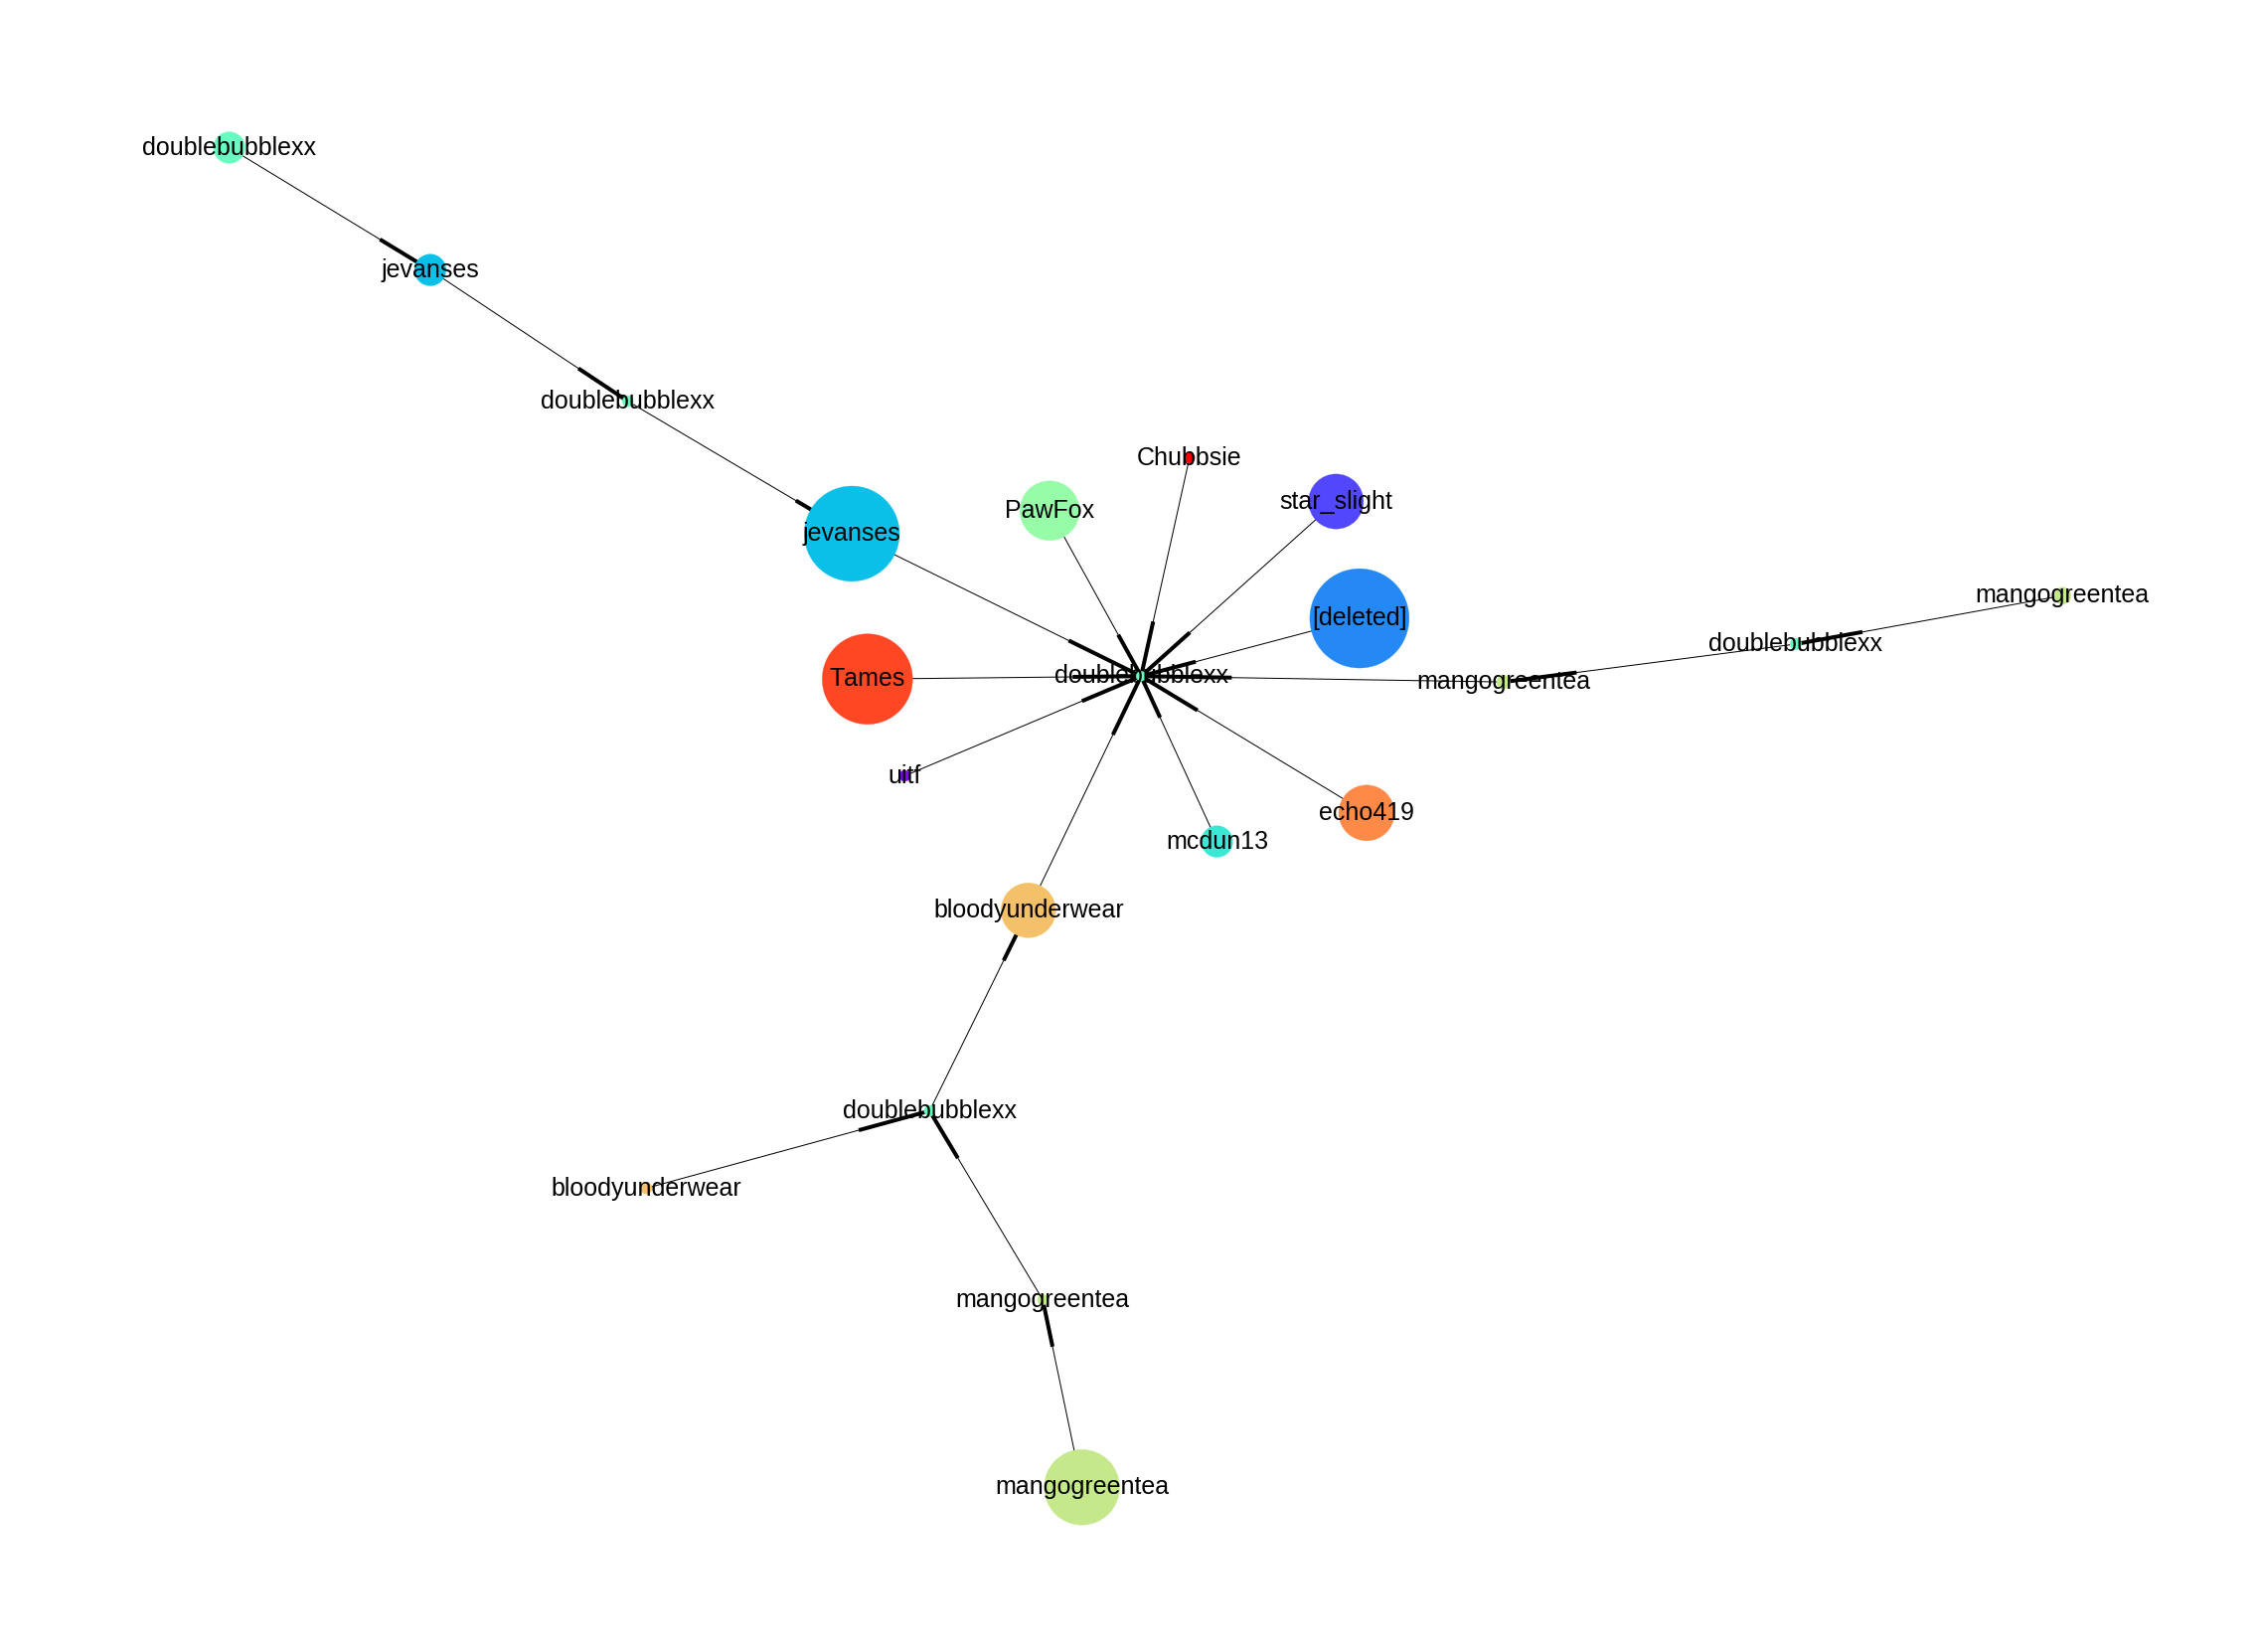
\includegraphics[width=0.45\textwidth, height = 5cm ]{Figures/ReplyGraphSW}
        \label{fig:rGraphSW}
    }
    \subfloat[]{
        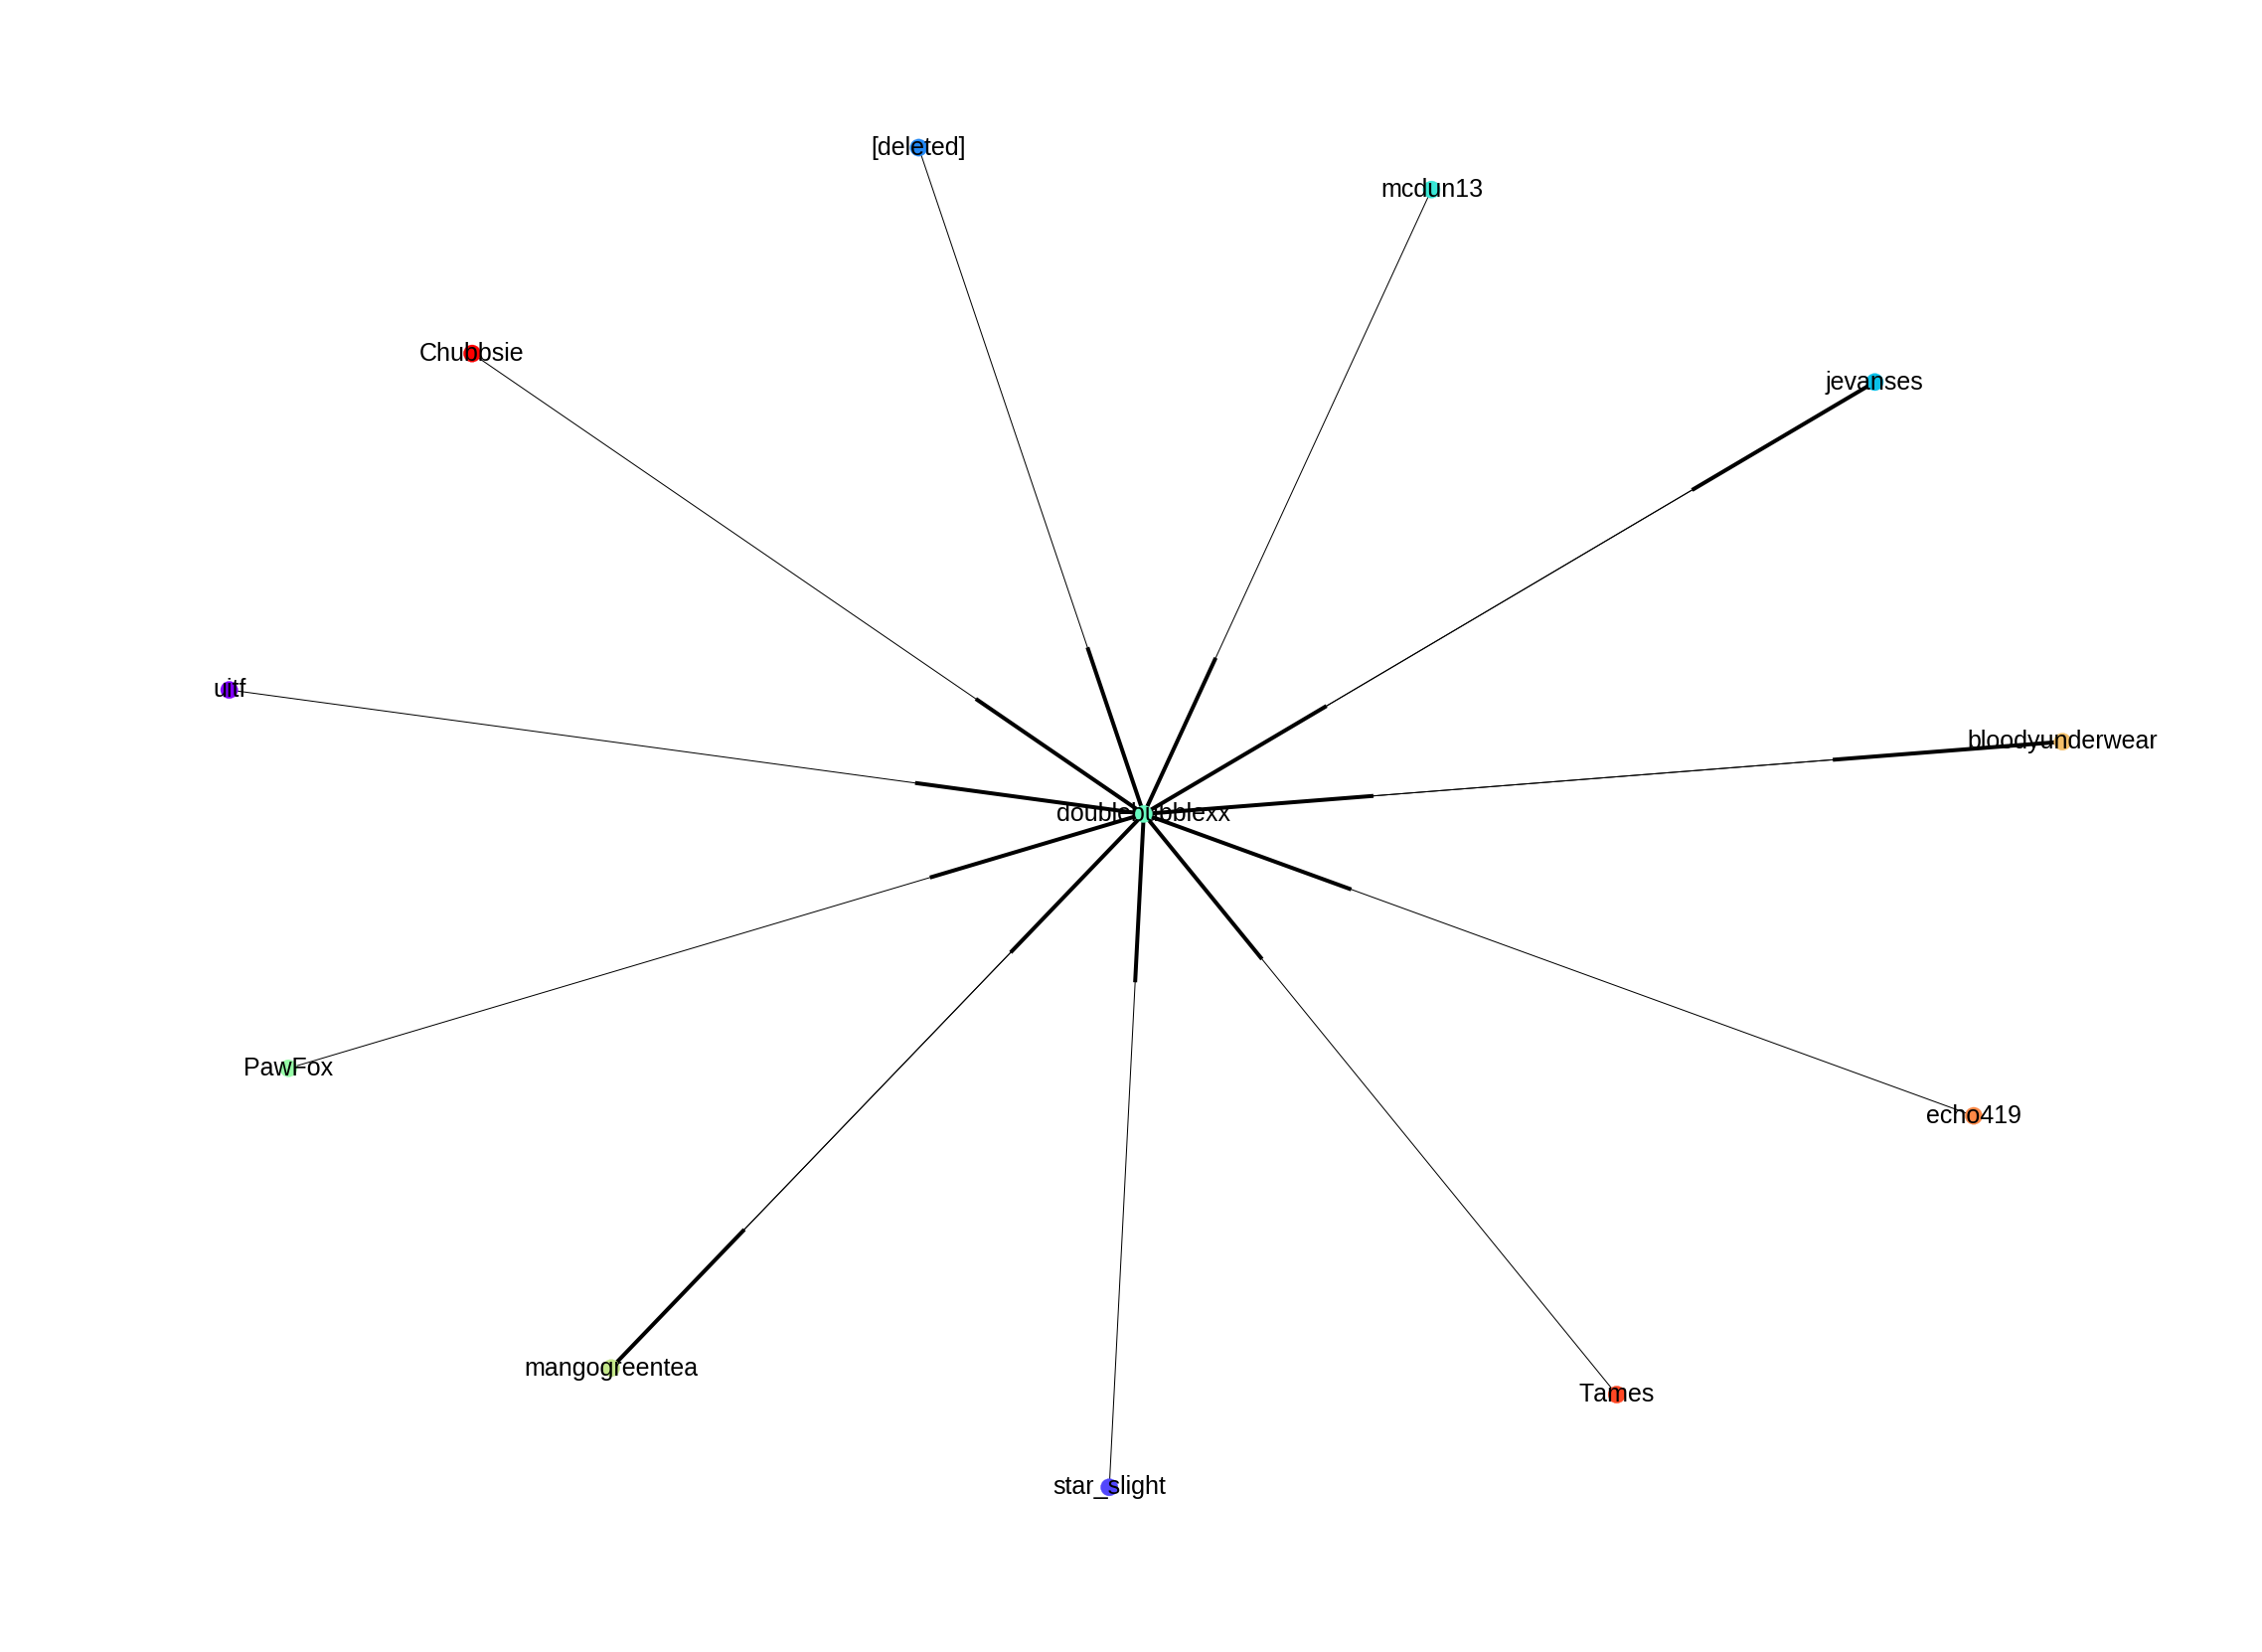
\includegraphics[width=0.45\linewidth, height = 5cm ]{Figures/UserGraphSW}
        \label{fig:uGraphSW}
    }
    
    
    \subfloat[]{
        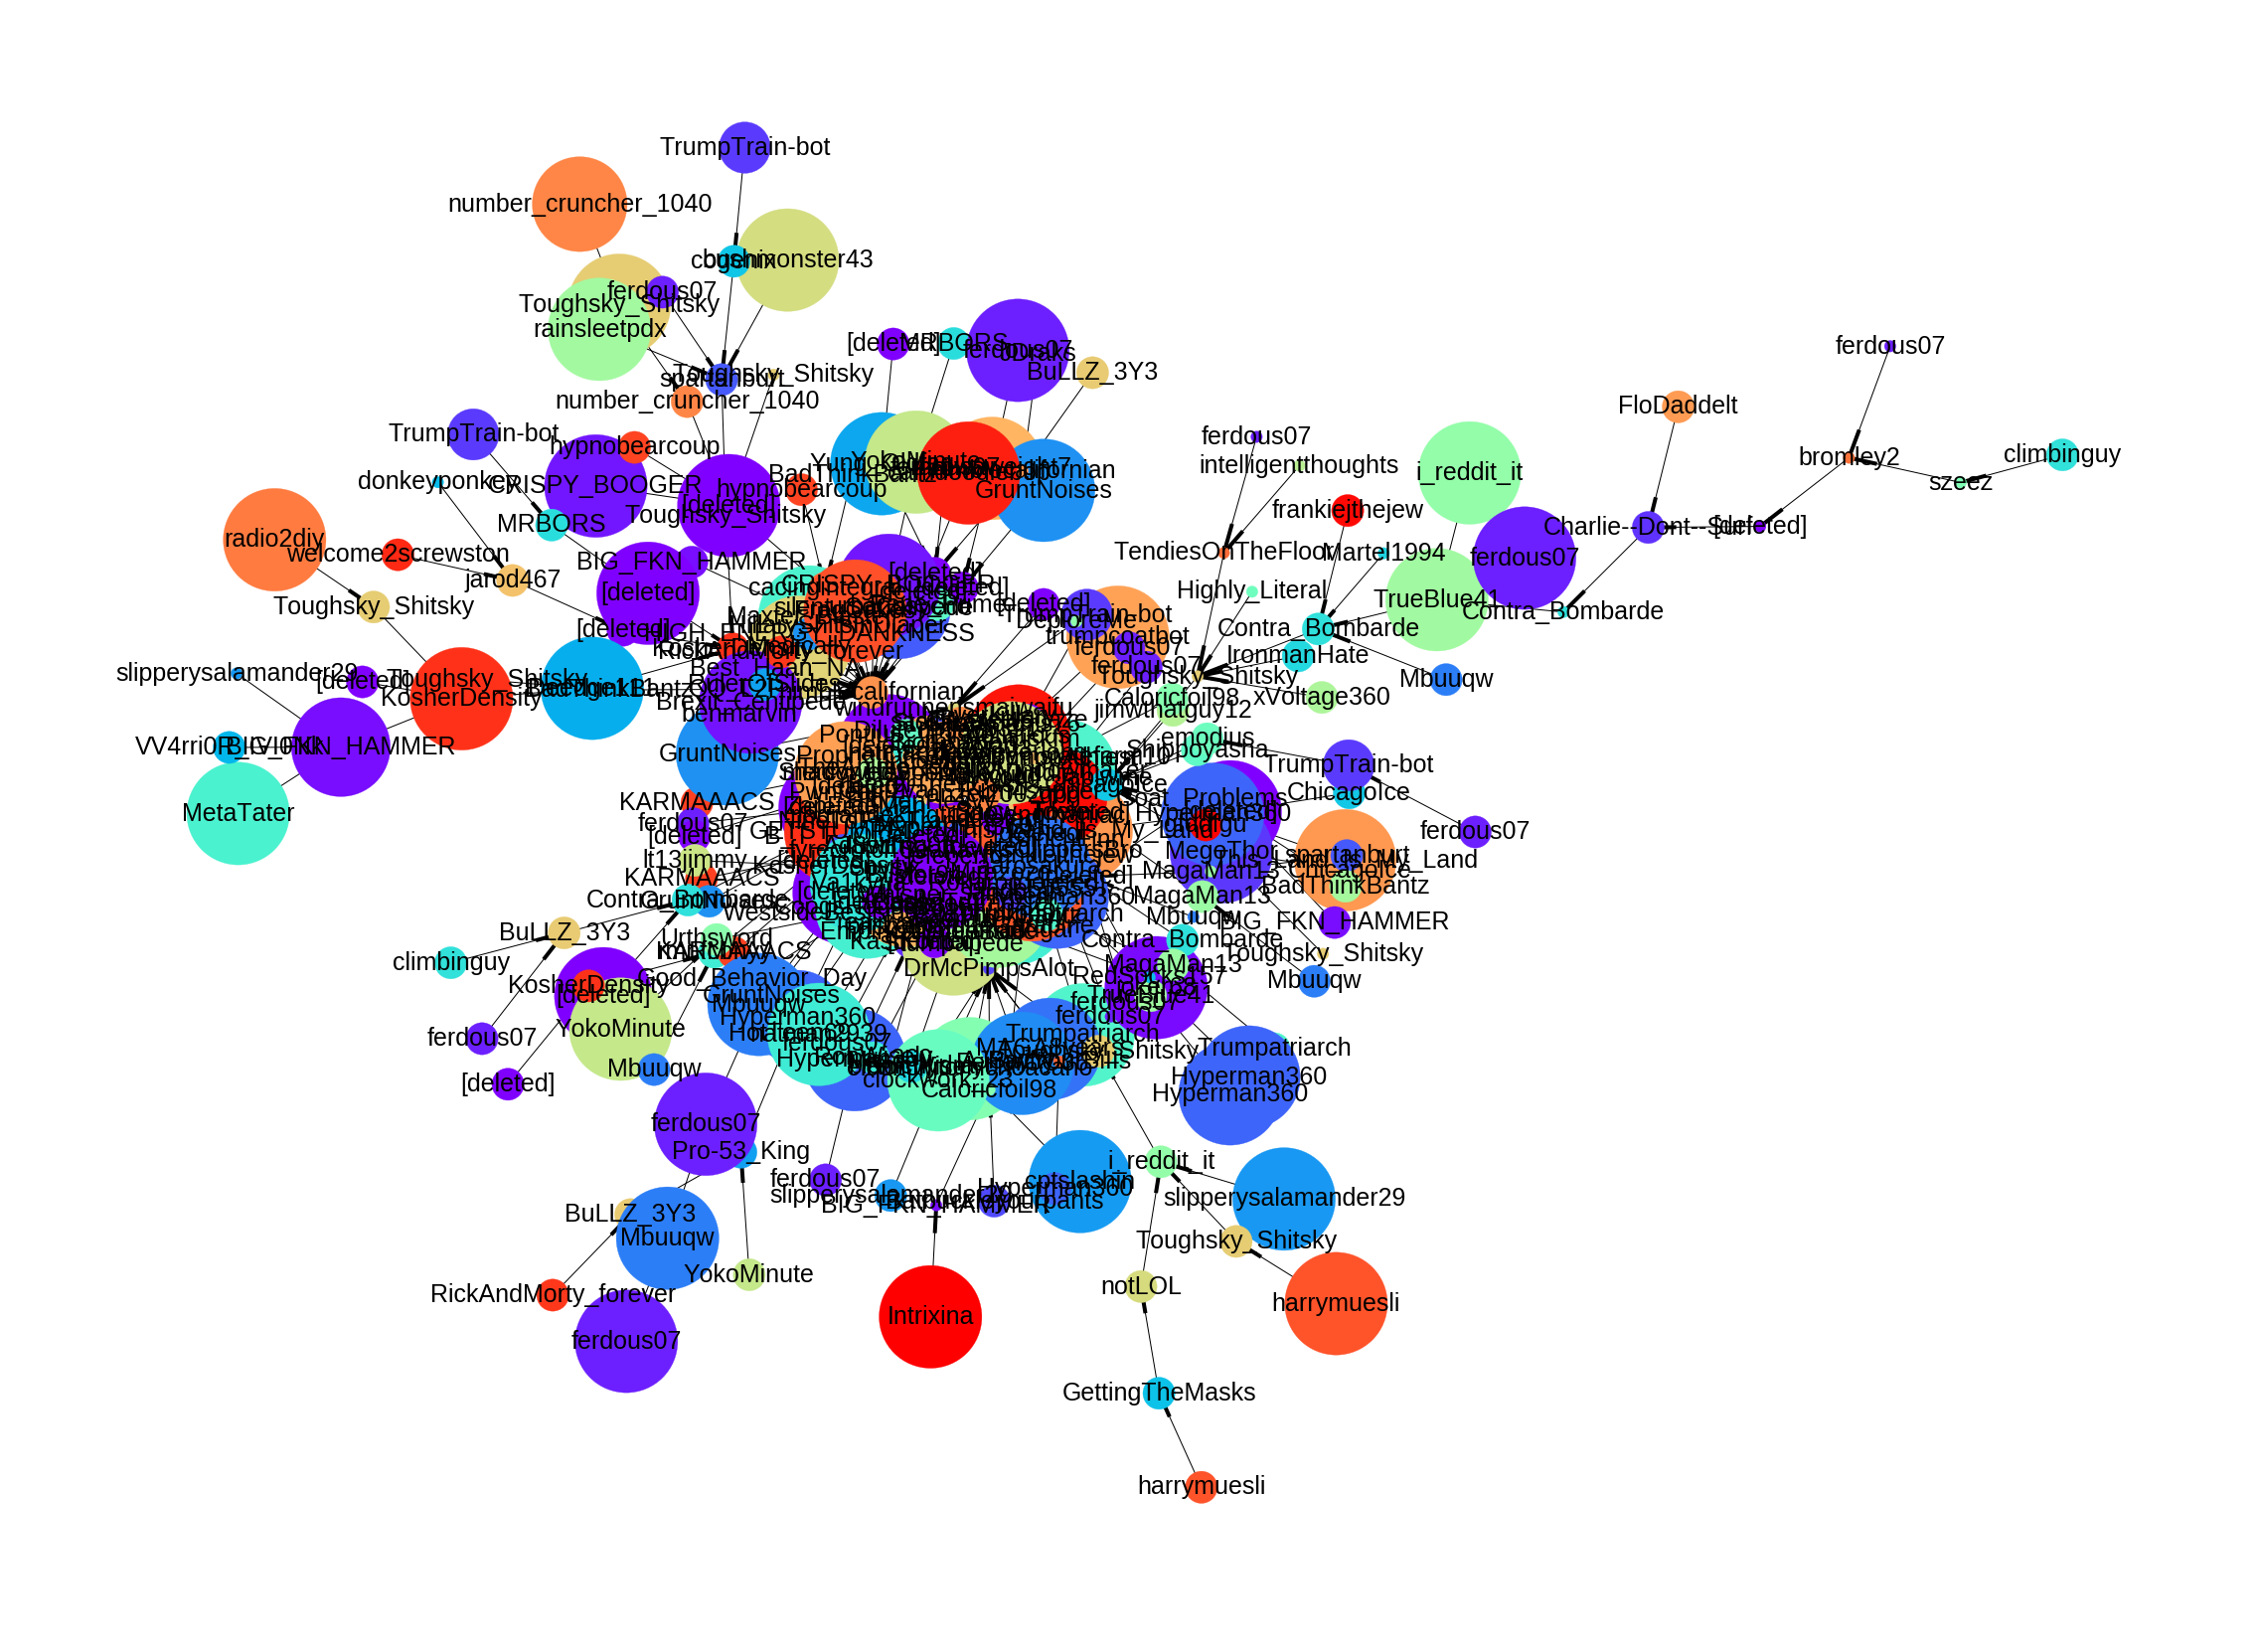
\includegraphics[width=0.45\linewidth, height = 5cm ]{Figures/ReplyGraphTD}
        \label{fig:rGraphTD}
    }
    \subfloat[]{
        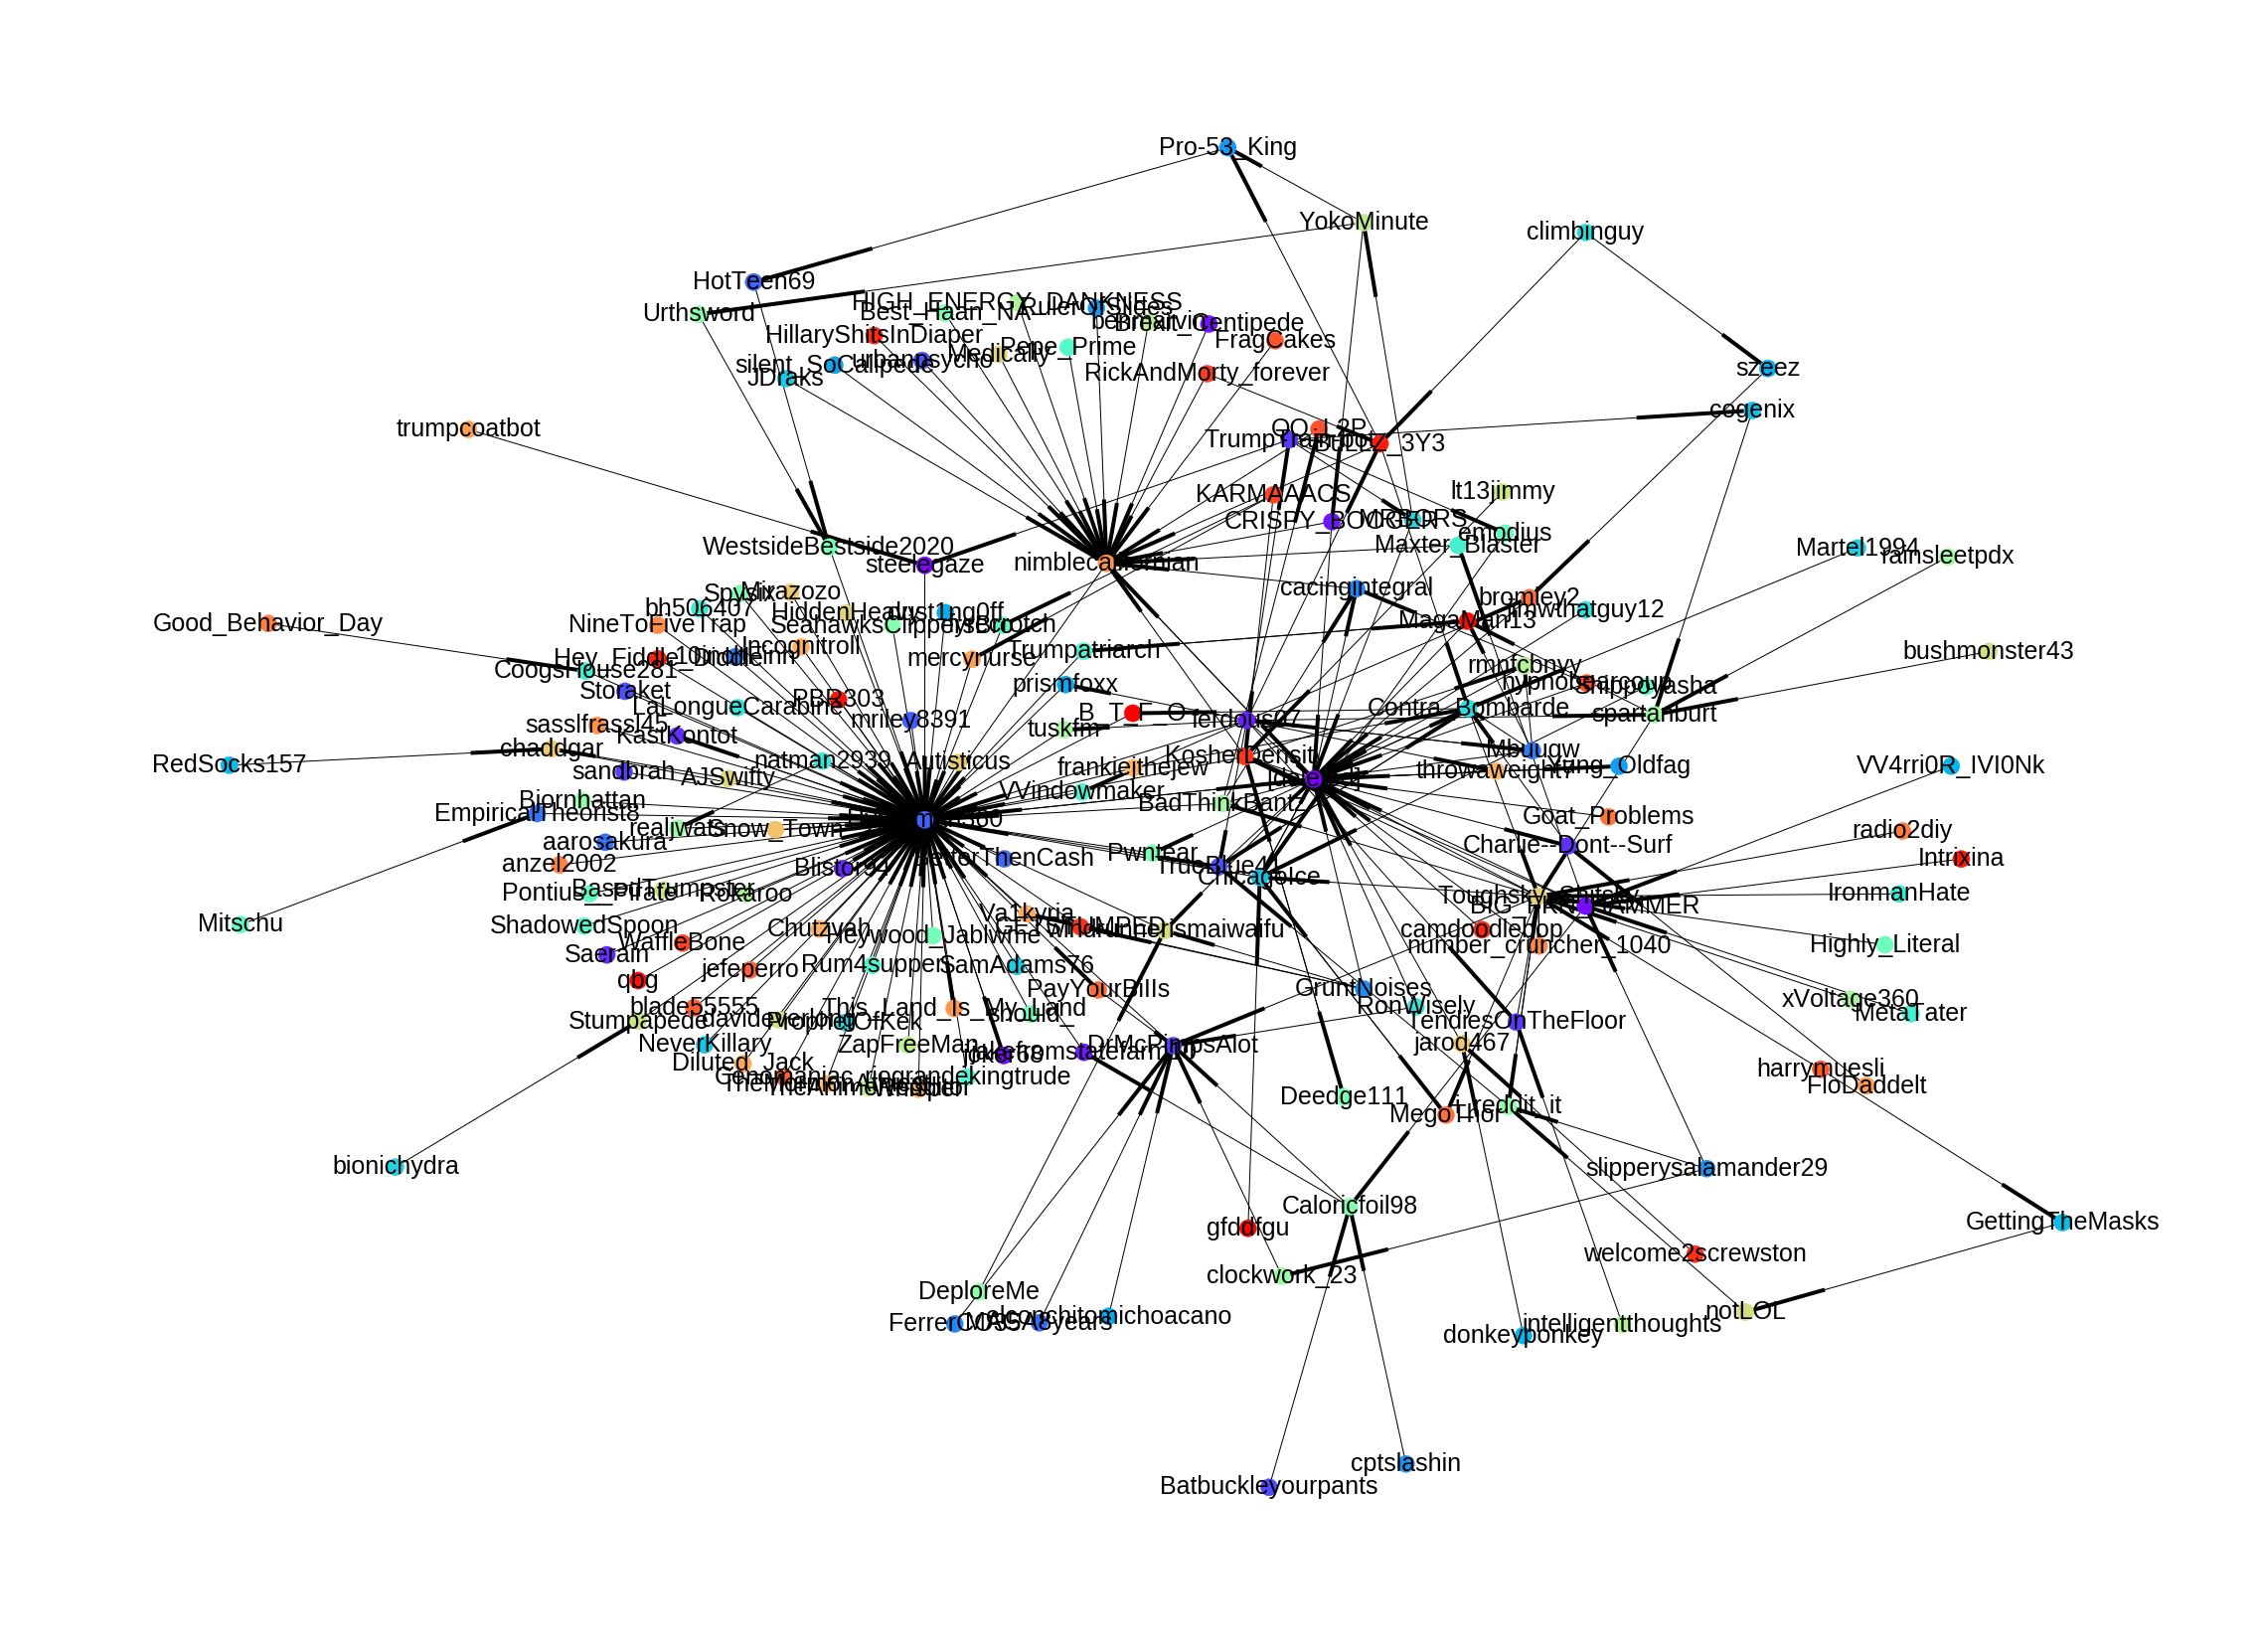
\includegraphics[width=0.45\linewidth, height = 5cm ]{Figures/UserGraphTD}
        \label{fig:uGraphTD}
    }
    \caption{ Example UserGraphs and their corresponding Reply graphs, Figure \ref{fig:uGraphSW} shows a random thread from the SW sub-reddit and \ref{fig:rGraphSW} shows the corresponding reply graph that arises from the response structure of the same thread. In comparison we have Usergraph Fig \ref{fig:uGraphTD} and its corresponding reply graph Fig \ref{fig:rGraphTD} from one of the Front page threads }
    \label{Fig:GraphExamples}
\end{figure*}



\subsubsection{Reply Graphs}
\label{Sec:Reply_graphs}
The first abstraction mimics directly the structure of conversation threads on Reddit. These abstractions are called Reply Graphs. We formulate a reply graph $R\{P,E,W\}$ as a thread of multi-layered posts in a thread in response to the root post $RP$ in the sub-reddit. Each graph $R$ consists of posts $P_i , P_j , i,j \in N$ , where N+1 is the total number of responses in the thread and Edges $E_{ij}$such that and Edge $E_{ij}$ exists $iff$ post $P_i$ was in response to post $P_j$ in the hierarchy of responses.  The weight of the edge $E_{ij}$ is found by calculating the cosine similarity between topic vector $T_i$ for post $P_i$ and the topic vector $T_j$ of post $P_j$. For a given dataset, the topic vectors are extracted using the model trained on that particular corpus ($LDA_{BL}$, $LDA_{SW}$).  This abstraction works well in modeling the conversational nature of these forums.  For convenience of the reader, we present a couple of example pairs from SW and Frontpage baseline datasets in Figure \ref{Fig:GraphExamples}

\subsubsection{Interaction Graphs}
\label{Sec:Interaction_graphs}
In this method, we represent each thread as a directed graph $G\{V,E,W\}$ where $V$ is the set of all users participating in a particular thread and $E$ are the directed  edges which correspond to interactions between two users $V_i , V_j  \in V$. The weight of each directed edge $E_{ij}$ corresponds to the average of all the edges between $V_i , V_j  \in V$ in the corresponding reply graph $R\{P,E,W\}$ as described above. This means that each reply graph is then mapped to a User graphs where the nodes are Users rather than posts. Another salient distinction between the two abstractions is that reply graphs resemble an n-ary tree and user graphs are directed cyclic graphs. 





\subsection{Macro and local metrics}
The abstractions are used to extract certain structural metrics from the conversation threads. These metrics are then used to validate structural differences in supportive conversations 


\subsubsection{Centrality}
For this metric we use the User Graphs. Node centrality is a metric that measures how central a node is in a network. It directly reflects the importance of the node when it comes to membership of the shortest connecting paths between all the nodes in the graph. More formally, we use betweenness centrality of a node which is defined as 
Betweenness centrality of a node $v$ is defined as 
$$
g(v) = \sum_{s \neq v \neq t}\frac{\sigma_{st}(v)}{\sigma_{st}}
$$
where $\sigma_{st}(v)$ is the total number of shortest paths from node $s$ to node $t$ and $\sigma_{st}$ is the number of those paths that pass through $v$. To understand whether the thread starters ($OP$) have a special place in the network, we evaluate both $OP$ centrality as well as median centrality across all the nodes in a User graph.

\subsubsection{Symmetrical users}
We define a symmetric user and a symmetric edges for user graphs. For a user $V_i$ in the user graph $G\{V,E,W\}$ as described in Section
, a symmetric user is a user who interacts with $V_o$ or the $OP$ and receives a response back from the $OP$. We find the fraction 
$$
U_{sym}=\frac{\textit{total number of symmetric users }}{\textit{Total users in a thread}}
$$

\subsubsection{Urgency}
To understand how Suicide watch subreddit users responds to the $OP$ and each other, compared to other sub-reddit threads on the frontpage, we calculate differences between the posting times between consecutive messages in a reply graph. We compute the median response times per thread, for $OP$'s posts and for all other posts. 

\subsubsection{Branching Factor}
Branching factor is a quantity that reflects the fan out of a conversation as it evolves.
To measure this phenomena, we use the reply graphs, which resemble a n-ary directed acyclic graph, to evaluate the branching factor. The branching factor is formally described as 
$$\tau = \frac{1}{|D|} \sum_{d \in D}^{} \frac{1}{|N_d|} \sum_{n\in N_d}^{} \textit{InDeg}(n)$$


\subsubsection{Response distance}
A user who interacts frequently with a thread, may contribute at different stages of hierarchy. Intuitively, for a one on one conversation to exist, the user needs to contribute back to the thread at alternate levels of hierarchy. To measure this phenomenon, we assume that a user $U$ contributes in a reply graph at variable depths $d_i \forall i \in [0,D]$. 
We calculate the average difference between two consecutive contributions $d_{avg}$
$$ d_{avg} = \frac{\sum_{i=0}^{D} d_{i+1} - d_i }{D}$$
We calculate the values of $d_{avg}$ for both $OP$ and other users in the thread.


\subsubsection{Semantic similarity}
\label{Topic}
We use a popular word embedding method called \textit{Word2Vec} \cite{mikolov2013distributed} which learns representations of a set of words from a corpus of text, which in our case is the text from Suicide Watch and baseline fora. These representations can be used to extract text embedding vectors for each post which belong to a $N$ dimensional space $R^N$




\subsection{Structural metrics}
\remSVi{This probably needs to be briefly introduced/explained earlier in the manuscript?}
To understand relation of local structure in conversations with its nature, we compare the quantity called \textsl{motif occurrence ratio}. After calculating motif census across the dataset\cite{Batagelj2001}, we select progressive subsets of graphs from both datasets with nodes $n \in [3 , 40]$. \remSVi{What is the motivation behind the 3-40 thresholds?} We test each graph for the frequency of occurance of the 16 possible triadic motifs as shown in Figure\ref{fig:motifs}. For each of these node values we get a subset of graphs with those specific number of nodes, from Suicide watch and baseline frontpage, lets call then $\Gamma_{SW}$ and $\Gamma_{BL}$. Let us assume that for a given value of $n$ , $\Gamma_{SW}$ has $K_{SW}$ graphs and $\Gamma_{BL}$ has $K_{BL}$ graphs. We then count for a given motif, number of occurrences in $\Gamma_{SW}$ and $\Gamma_{BL}$ where the graph had at-least one instance of that motif. Let us call the total number of graphs in $\Gamma_{BL}$ with a given motif as $\gamma_{BL}$ and $\gamma_{SW}$ likewise for the $\Gamma_{SW}$ graphs. 
We then define the motif occurrence ratio as the fraction values for $\frac{\gamma_{BL}}{K_{BL}}$ and $\frac{\gamma_{SW}}{K_{SW}}$ for all the 16 motifs across all the chosen values of $n$. 


\begin{figure*}[!h]
	\centering
	% \hspace*{-5mm}
	\subfloat[]{
		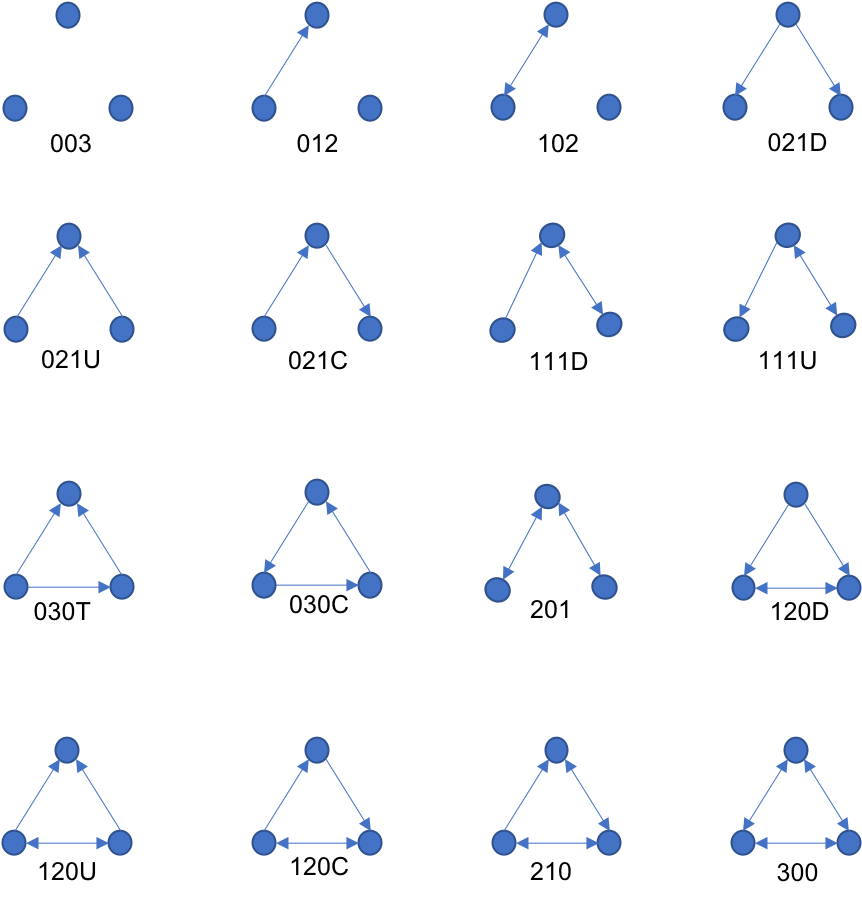
\includegraphics[width=0.7\textwidth]{Figures/TriadVariants}
		\label{fig:motifs}
	}
    
	\subfloat[]{
		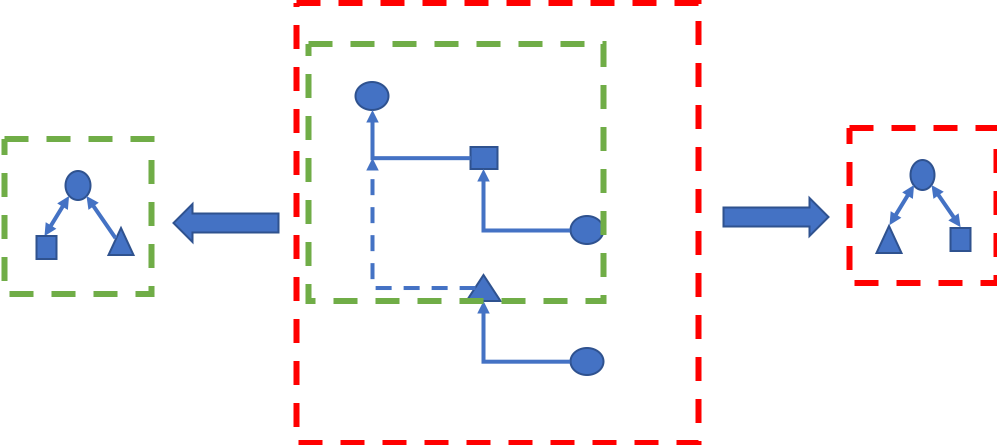
\includegraphics[width=0.7\linewidth, height = 5cm ]{Figures/thread}
		\label{fig:motifStruct}
	}
\caption{ Figure \ref{fig:motifs} shows the 16 different types of motifs that are looked for in the user graph data. Figure \ref{fig:motifStruct} shows how three unique users could produce different motifs. The three shapes represent different users and the dotted line means the message order is irrelevant.}
	\label{Fig:motifs}
\end{figure*}

